\documentclass[border=8pt]{standalone}
\usepackage{tikz}
\usepackage{amsmath, amssymb, bm}
% UiO colour palette and shared TikZ styles for thesis flowchart figures.
% Input by every standalone TikZ figure in this directory.

% UiO colours
\definecolor{uioblue1}{RGB}{62, 49, 214}
\definecolor{uioblue2}{RGB}{134, 164, 247}
\definecolor{uioblue3}{RGB}{230, 236, 255}
\definecolor{uiogreen1}{RGB}{46, 196, 131}
\definecolor{uiogreen2}{RGB}{108, 225, 171}
\definecolor{uiogreen3}{RGB}{206, 255, 223}
\definecolor{uioorange1}{RGB}{254, 161, 27}
\definecolor{uioorange2}{RGB}{253, 203, 135}
\definecolor{uioorange3}{RGB}{255, 232, 212}
\definecolor{uiopink1}{RGB}{222, 0, 0}
\definecolor{uiopink2}{RGB}{251, 102, 102}
\definecolor{uiopink3}{RGB}{254, 224, 224}
\definecolor{uioyellow}{RGB}{255, 254, 167}
\definecolor{uiogray}{RGB}{178, 179, 183}

\usetikzlibrary{arrows.meta, positioning, calc, fit, backgrounds}

% Shared styles
\tikzset{
  % Generic card with a coloured accent (#1 = base hue).
  card/.style 2 args={
    rectangle, rounded corners=3pt,
    draw=#1, line width=0.55pt,
    fill=#2,
    inner xsep=8pt, inner ysep=7pt,
    align=center,
    font=\small,
    text=black!85,
  },
  card-blue/.style  ={card={uioblue1}{uioblue3}},
  card-green/.style ={card={uiogreen1}{uiogreen3}},
  card-orange/.style={card={uioorange1}{uioorange3}},
  card-pink/.style  ={card={uiopink1}{uiopink3}},
  card-gray/.style  ={card={black!55}{black!4}},
  % Central focus body (heavier border, white fill).
  hub/.style={
    rectangle, rounded corners=8pt,
    draw=black!75, line width=0.9pt,
    fill=white,
    inner xsep=10pt, inner ysep=10pt,
    align=center,
    font=\small,
  },
  % Title text on each card.
  card-title/.style={font=\small\bfseries, text=black!85},
  % Arrows.
  flow/.style 2 args={
    -{Stealth[length=2.2mm, width=1.8mm]},
    line width=0.8pt,
    draw=#1,
    color=#1,
  },
  flow-blue/.style   ={flow={uioblue1}{uioblue1}},
  flow-green/.style  ={flow={uiogreen1!85!black}{uiogreen1!85!black}},
  flow-orange/.style ={flow={uioorange1!90!black}{uioorange1!90!black}},
  flow-pink/.style   ={flow={uiopink1}{uiopink1}},
  flow-gray/.style   ={flow={black!55}{black!55}},
  % Edge labels — small, white background, role colour.
  edge-label/.style={
    font=\scriptsize,
    fill=white, inner xsep=2pt, inner ysep=1pt,
  },
}


\begin{document}
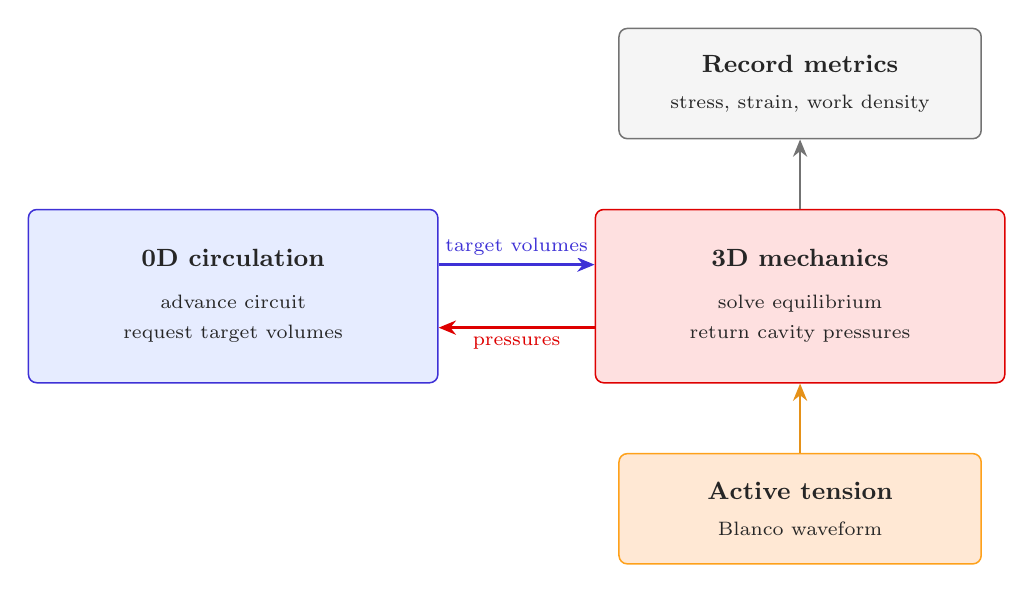
\begin{tikzpicture}[x=1cm, y=1cm]

  % Main pair on a horizontal axis.
  \node[card-blue, minimum width=52mm, minimum height=22mm] (circ) at (-3.6, 0) {%
    {\bfseries 0D circulation}\\[4pt]
    \scriptsize advance circuit\\
    \scriptsize request target volumes%
  };
  \node[card-pink, minimum width=52mm, minimum height=22mm] (mech) at ( 3.6, 0) {%
    {\bfseries 3D mechanics}\\[4pt]
    \scriptsize solve equilibrium\\
    \scriptsize return cavity pressures%
  };

  % Output above mechanics.
  \node[card-gray, minimum width=46mm, minimum height=14mm] (rec) at (3.6, 2.7) {%
    {\bfseries Record metrics}\\[2pt]
    \scriptsize stress, strain, work density%
  };

  % Input below mechanics.
  \node[card-orange, minimum width=46mm, minimum height=14mm] (act) at (3.6, -2.7) {%
    {\bfseries Active tension}\\[2pt]
    \scriptsize Blanco waveform%
  };

  % Bidirectional volumes/pressures exchange.
  \draw[flow-blue, line width=1.0pt]
    ([yshift=4mm]circ.east) --
    node[edge-label, text=uioblue1, above=2pt, pos=0.5] {target volumes}
    ([yshift=4mm]mech.west);
  \draw[flow-pink, line width=1.0pt]
    ([yshift=-4mm]mech.west) --
    node[edge-label, text=uiopink1, below=2pt, pos=0.5] {pressures}
    ([yshift=-4mm]circ.east);

  % Active tension drives mechanics; mechanics emits metrics.
  \draw[flow-orange] (act) -- (mech);
  \draw[flow-gray]   (mech) -- (rec);

\end{tikzpicture}
\end{document}
